\begin{usecase}{View Integrated Calendar}
    \ucbasicinfo{High}{Regular}
    \ucshortdescription{This UC allows the user to view their calendar events from all configured calendars through iOS's native calendar system.}
    \uctrigger{This UC is triggered when the user opens the calendar view in the app.}
    \ucactors{User}{EventKit}
    \ucpreconditions{
        \begin{itemize}
            \item User must be logged in
            \item User must have granted calendar access permission
            \item User must have at least one calendar configured in iOS
        \end{itemize}
    }
    \ucrelationships{N/A}{N/A}{N/A}
    \ucinputsoutputs{
        \begin{itemize}
            \item \textbf{Calendar view preferences} (Source: User)
            \item \textbf{Calendar events} (Source: iOS Calendar System)
        \end{itemize}
    }{
        \begin{itemize}
            \item \textbf{Integrated calendar view} (Destination: App)
        \end{itemize}
    }
    \ucmainflow{
        \begin{enumerate}
            \item The user opens the calendar view in the app.
                  \ucinfo{The app uses EventKit to fetch events from all configured calendars.}
            \item The app displays the integrated calendar view.
                  \ucinfo{Events from all calendars are shown in a unified view.}
            \item The user can interact with the calendar view.
                  \ucinfo{The user can view event details, switch between different view modes (day, week, month), and filter calendars.}
        \end{enumerate}
    }
    \ucalternateflows{
        \begin{itemize}
            \item If no calendars are configured, the app shows an empty state with instructions to add calendars through iOS settings.
            \item If calendar access is revoked, the app prompts the user to grant access in iOS settings.
        \end{itemize}
    }
    \ucexceptions{
        \begin{itemize}
            \item \textbf{Calendar access denied:} If the app doesn't have calendar access permission.
            \item \textbf{Event fetch failure:} If EventKit fails to retrieve calendar events.
        \end{itemize}
    }
    \ucconclusion{The UC ends when the user has a clear view of their calendar events from all configured calendars.}
    \ucpostconditions{The user can view and interact with events from all their configured calendars in a unified interface.}
\end{usecase}

\begin{figure}[!h]
    \centering
    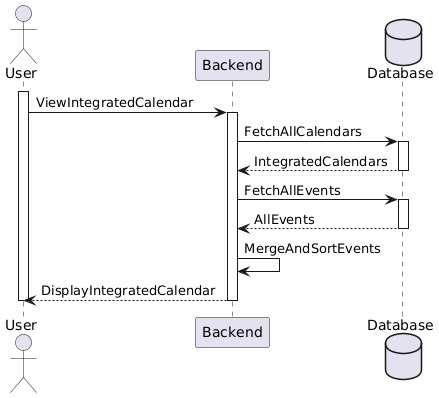
\includegraphics[width=0.5\textwidth]{images/docs/diagrams/sequence-diagrams/all-sequence-diagrams/View Integrated Calendar.png}
    \caption{View Integrated Calendar Sequence Diagram}
    \label{fig:seq/view-integrated-calendar}
\end{figure}

The ``View Integrated Calendar Sequence Diagram'', shown in \textbf{Figure~\ref{fig:seq/view-integrated-calendar}}, illustrates how the app uses EventKit to fetch and display calendar events from iOS's native calendar system.

The process involves:
\begin{enumerate}
    \item The app requests calendar events through EventKit when the user opens the calendar view
    \item EventKit fetches events from all configured calendars in iOS
    \item The app displays the events in an integrated view
    \item The user can interact with the events and switch between different view modes
\end{enumerate}

This approach leverages iOS's built-in calendar infrastructure to provide a seamless calendar viewing experience.